\chapter{Zedboard}
\label{ch:zedboard}

After having failed to boot VxWorks on the Cyclone V and waiting for Quartus licence, we decided to try to boot the same RTOS on the Zedboard, a Zynq-7000 based board.\\
This board was chosen because we have seen that it has official documentation 
and guides and it’s one of the boards supported by VxWorks. \\
Moreover there are programs like Vivado to develop and debug software.

\section{Overview}
\begin{figure}[h]
	\centering		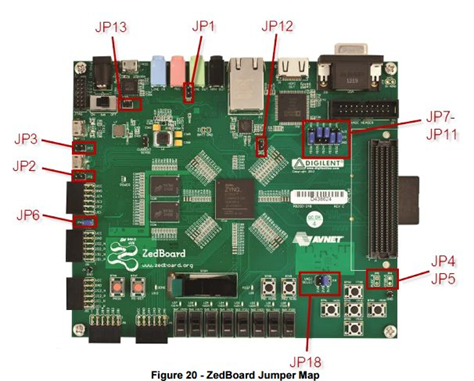
\includegraphics[width=0.8\textwidth]{img/zedboard}
	\caption{Zedboard}
    	\label{fig:zedboard}
\end{figure}

\begin{itemize}
\item SD Card;
\item 512 MB DDR3 (128M x 32) o 256 Mb QSPI Flash;
\item USB 2.0 FS USB-UART bridge;
\item Dual ARM Cortex-A9 MPCore Up to 667 MHz.
\end{itemize}


\section{Building the kernel image}
We have built the kernel image with Windriver workbench following this guide:\\
\href{https://www.xilinx.com/support/documentation/application_notes/xapp1158-zynq-7000-vxworks-bsp.pdf}{Guide}\\
We created the .bif file with the following format:

\begin{lstlisting}[style=myCode]
ZC702_bif_for_VxWorks: 
{ 
[bootloader]zynq_fsbl_0.elf 
bootROM.elf 
}
\end{lstlisting} 
And downloaded the .elf file from the official Xilinx website.

\section{Generating the bootloader}
We built the bootloader using the Vivado TCL shell using “bootgen” following this guide \url{http://www.wiki.xilinx.com/Prepare+boot+image} omitting the “I” parameter  because was not recognised.\\

\begin{figure}[h]
	\centering		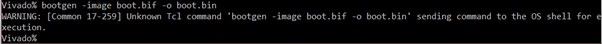
\includegraphics[width=0.8\textwidth]{img/bootloaderbuild}
	\caption{Bootloader build}
    	\label{fig:bootloaderbuild}
\end{figure}

\subsection{Bootloader}
\begin{figure}[h]
	\centering		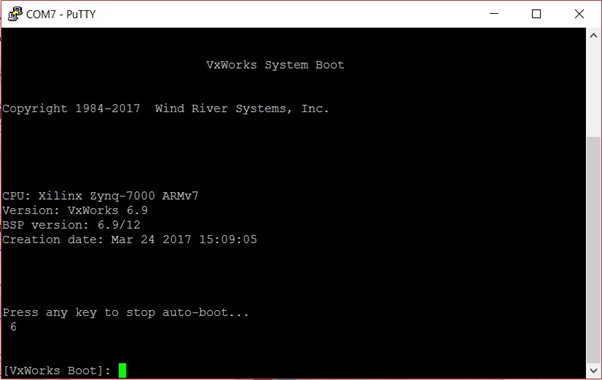
\includegraphics[width=0.6\textwidth]{img/boot}
	\caption{Boot}
    	\label{fig:boot}
\end{figure}

We installed the Cypress drivers for the serial interface.\\
We copied boot.bin e vxWorks on the SD card and connected with Putty. \\
The bootloader started up.

\subsection{Bootloader configuration}
We stopped the autoboot, then we inserted the following instructions as suggested  from the guide:\\
\href{https://www.xilinx.com/support/documentation/application_notes/xapp1158-zynq-7000-vxworks-bsp.pdf}{Guide}

\begin{figure}[h]
	\centering		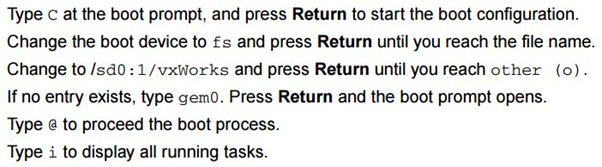
\includegraphics[width=0.8\textwidth]{img/code}
	\caption{Code}
    	\label{fig:code}
\end{figure}

\subsection{Errors and bugs}
After some attempts it gave us the following error\\

\begin{lstlisting}[style=myCode]
Host Name: bootHost
Target Name: vxTarget
User: target
ERROR: ipcom_drv_eth_init: drvname:, drvunit: 0
0x1100e5c (tRootTask): task 0x1100e5c has had a failure and has been stopped.
0x1100e5c (tRootTask): fatal exception in a kernel task or stack overflow!
Instantiating /sd0:0 as rawFs,  device = 0x10001
\end{lstlisting} 

We noticed that the parameters inserted previously are not stored in the SD but in internal memory. So resetting, rebooting, formatting the SD and installing Linux had no effect in deleting those values.

\section{XMD console}
We used the Xilinx SDK (Software development kit), a software installed with Vivado, used to develop embedded applications.\\
We tried to put the bootloader and the image directly in RAM with the XMD console included in the SDK.\\
Trying to connect with the connect command we have discovered that 2 usb cable were needed: the first for the serial, the second connected to the PROG port.

\subsection{Connected to the board}
Following this guide \url{https://www.xilinx.com/support/documentation/sw_manuals/xilinx2014_1/ug1043-embedded-system-tools.pdf} pg.73, we inserted the command “connect arm hwCortexA9” without result.\\
Following the help of the console we discovered that the right command is “connect arm hw”.\\

\begin{figure}[h]
	\centering		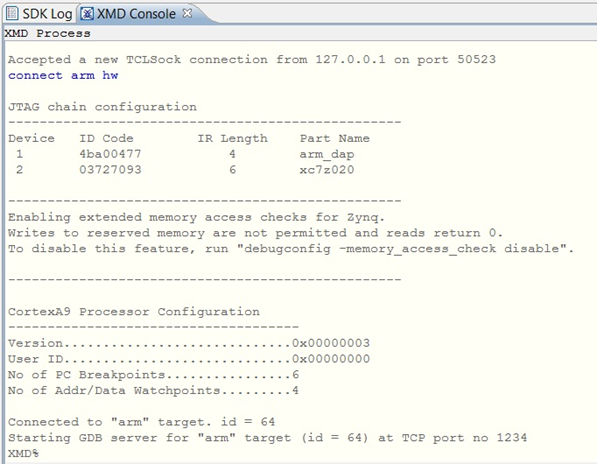
\includegraphics[width=0.6\textwidth]{img/xmdconnect}
	\caption{XMD connect}
    	\label{fig:xmdconnect}
\end{figure}


\subsection{RAM busy}
Once connected we tried to put the files directly in RAM. we executed the command “dow -data boot.bin 0x00100000” giving us the following error:

\begin{lstlisting}[style=myCode]
AP transaction error (DP CTRL_STAT=0xf0000021)
Error Address = 0x00100000, Size = 0x00000004
\end{lstlisting}

We discovered that the problem wasn’t the register but the fact that the processor was not stopped and the memory was busy

\subsection{Missing component}
We tried to manually stop and reset the processor with “stop” and “rst” commands. After some researches we discovered that ps7\_init.tcl was missing. We downloaded it and we used it to stop the processor:


\begin{lstlisting}[style=myCode]
source ps7_init.tcl
ps7_init
ps7_post_config
stop
\end{lstlisting}

\subsection{Directly in RAM}
We were able to stop the processor and to put the files in RAM with the “dow” command. Then we gave the “con”  and “run” command but nothing showed up in Putty. 

\begin{lstlisting}[style=myCode]
XMD% con

RUNNING> XMD%
\end{lstlisting}

After this we asked help on the knowledge forum to resolve the stackoverflow problem but no one was able to help us 
\url{https://ask.windriver.com/en/questions/35789/zedboard-boot-vxworks-69-problem/}.



 


















